\chapter{Applications}

The qubits control system developed within this thesis can be used for various experiments in different quantum technology fields.
Although the integration in \Qibolab is focused on quantum computing, the final objective is to have a complete instrument able to fully control of a qubit state.
So it is possible to imagine also non-computing applications.

In any case, let's focus on the two main applications where \Qibosoq could be useful and could be used in the short term. These are:
\begin{itemize}
    \item in quantum computing, for quantum machine learning applications.
    \item in quantum sensing, in particular for the QubIT project;
\end{itemize}


\section{Quantum machine learning: determining probability density functions}
\label{sec:qml_application}

The RFSoC-based control system that was developed for this thesis has already been used in quantum machine learning applications, in particular to fit probability density functions~\cite{Robbiati2023}.

This is a relevant short-term application because even a single not-optimally-tuned qubit can be work fine.

To the reader, using a quantum computer for fitting, might seem useless. 
It is a fair doubt, but there are still situations where the analytical underlying distribution is not known and the problem cannot be efficiently solved classically.

For example, the reliable determination of probability density functions (PDF) from data samples is still an active research topic in studies of fundamental physics.\\
With quantum computing and, specifically, adiabatic evolution algorithms, it is possible to approximate the underlying distribution via a circuit-based quantum device.

Given a one-dimensional function $f(t)$ with $t\in [0, T]$, we can build a regression model by choosing an observable such that two Hamiltonans $H_0$ and $H_1$ exist and respect the condition of having their ground state energy as the two values defining the range to which the function will be bounded.

We can then interpret the regression problem as the search for a time dependent Hamiltonian such that its ground state energy evolves as $f(t)$:
\begin{equation}
    \left< H(t) \right> = f(t)
\end{equation}

The Hamiltonian can be also written in terms of a new function $s(t; \theta)$, called \textit{scheduling function}, that describes a variational circuit defined by a set of parameters $\theta$:

\begin{equation}
    H(t) = [1 - s(t; \theta)]H_0 + s(t;\theta) H_1
\end{equation}

In this way, the problem is reduced to finding the right parameters $\theta$.

The complete, schematic, procedure is at follows:

\begin{enumerate}
    \item we generate a sample of variables $\{x\}$ from a chosen distribution;
    \item we compute the empirical \textit{cumulative density function} (CDF) from the extracted samples;
    \item we select $N_{train}$ data samples such that their values match some of the evolution times controlled by $s$;
    \item we map each pair $(x_i, f_i)$ into $(\tau_i, E_i)$ with the second pair representing two generic values of the evolution time/energy of the target observable evaluated at the evolved state with $\tau = t/T$;
    \item we define a loss function to minimize as:
        \begin{equation}
            J = \frac{1}{N_{train}} \sum_{j=1}^{N_{train}} (f_j - E_j (\theta))^2
        \end{equation}
        It is important to have a monotonic regression function, eventually, we could add extra penalty terms that, increasing with $j$, would assure the monotony; 
    \item we perform a training of the parameters $\theta$ to minimize the loss function. This can be done with classic, quantum or hybrid schemes.
\end{enumerate}

\begin{figure}[ht]
    \centering
    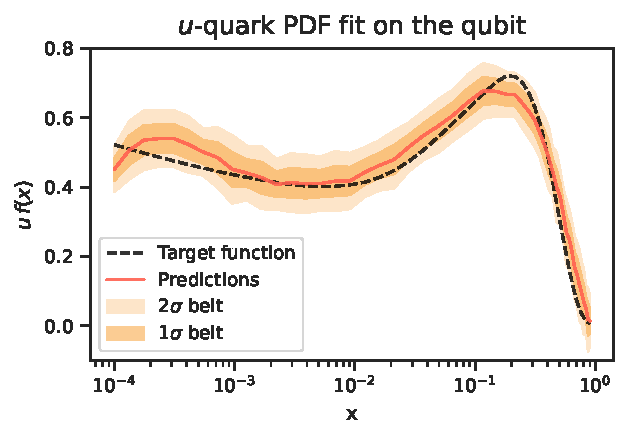
\includegraphics[width=0.6\textwidth]{Other sections/figures/qpdf.pdf}
    \caption{PDF of the $u$-quark, fitted with the QML model with a \Qibosoq-controller RFSoC.}
    \label{fig:updf}
\end{figure}

As example, we take some data samples from the NNPDF4.0~\cite{Ball2022} PDF grid.
Using a variational ansatz composed of consecutive rotations~\cite{PrezSalinas2020}, we encode the values of $x$ and proceed with the optimization minimising the MSE using the ADAM~\cite{adam} optimizer.
In this case, the optimization was done partially on classical hardware,  as a pre-training, and part on a TII single qubit device controlled by \Qibosoq.

In \cref{fig:updf}, an example of a plot obtained with this procedure is presented.
Both the expected PDF and the fitted one, with \Qibosoq and the \RFSoC, are presented.


\section{Quantum sensing applications}
\label{sec:sens_application}

For the moment, \Qibosoq has not been used in sensing applications, but it has been designed to be flexible and to support different kind of applications, from the circuits-based QML that we saw in last section to more pulse-based optimization protocols (for optimal-control, for examples) or for sensing applications.

What are the special needs of quantum sensing, from a control device / software point of view?\\
It is difficult to have a complete list of required features, but we could say that the main elements are:
\begin{itemize}
    \item extensive control of the pulses to execute (shaping, timing, frequency modulation, phases etc.);
    \item fast and precise acquisition;
    \item support for continuous measurements;
    \item good scaling properties;
    \item support for highly multiplexed systems;
\end{itemize}

\Qibosoq natively has, leveraging different \Qick functionalities, most of these characteristics.

In particular, through the Python API, the user has total control of the pulses and can both work optimizing speed and dead times, by leveraging all the pre-defined pulse shapes included in \Qibosoq, or focusing on optimal control, by defining in the client specific pulses from their IQ values.

The intrinsic characteristic of a RFSoC system give full control and flexibility on the frequency requests. 
In particular, when comparing the three currently supported Xilinx boards with the other commercial systems available for control at TII (Qblox, Quantum Machines, Zurich Instruments) the bandwidth of a single RFSoC channel (that can go above $10$ GHz) is not-comparable in respect to the standard bandwidths of $\approx200$ MHz (without local oscillators).
This speeds up \textit{incredibly} any experiment where there is the need to probe very different frequencies.

Currently, \Qick does not support continuous measurements and this reflects on \Qibosoq with the same limitation.
The problem, from the point of view of \Qick, stands in the use of memory that quickly fills the buffer size defined in FPGA logic.
Even tho this is a big limitation for sensing application, it is partially patchable through \Qibosoq.
Since \Qibosoq can be included easily in any Python client and is designed to minimize any latency, it should be possible to apply repeated measurement windows one after the other, without loosing excessive statistics in between them.\\
In any case, this issue should be taken into account and precisely measured for any real application of rare phenomena.

Regarding the scaling capabilities, the \Qick team is currently updating their firmwares so the is possible to synchronize different RFSoCs and use them collectively \textit{as a cluster-like system}.
The main \Qick developers admitted that this firmware upgrade will cause some problem in the \Qick software department: indeed the current proposed way of managing a RFSoC directly with \Qick involves a direct connection to the board, this is not possible when dealing to multiple boards at the same time.
In this problem, the \Qibosoq layout offers an easy solution: having already an external client responsible of managing communication with the board(s), it should be easy to give to it the new responsibility of splitting the program into different subsection for the different boards.

The high multiplexablity is a concept that, for qubits, has not really been under development.
However, \Qick has specific firmwares to control highly multiplexed arrays of Microwave Kinetic Inductance Detector~\cite{Magniez2022}, often referred to as MKIDs, (up to 4096 detectors with a single board). 
Although at the moment, the \Qibosoq development has been focused on qubit control, so it does not support this special firmware, it has been designed with flexibility as one of the main priority, since we knew from the start that \Qick would be upgraded independently from it and possibly without much interest in preserving backwards compatibility.\\
Thanks to this, it should not be difficult to extend support for the MKIDs firmware, although no development has yet been done in this direction.

\subsection*{Photon counter for dark matter detection}

As a theoretical example of quantum sensing application, we can take an experiment for axions detection~\cite{Dixit2021}.

In this section, we will present the code required to replicate the experiment, showcasing how a complex experiment can become trivial using the \Qibosoq API.
The experiment itself requires a hardware setup that stops me to be able to actually replicate it now, but still is a good example of how easily the implementation can become.

\begin{figure}[ht]
    \centering
    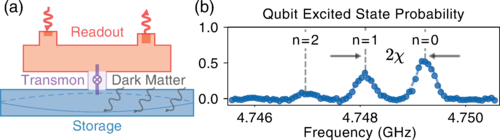
\includegraphics[width=0.6\textwidth]{Other sections/figures/dixit_setup.png}
    \caption{Hardware setup required of the axion-detection experiment.}
    \label{fig:dixit_setup}
\end{figure}

This hardware setup is presented in \cref{fig:dixit_setup} (a). 
The detection system requires a superconducting qubit (transmon) used as a bridge between a readout resonator (in the image depicted as a cavity) and an additional storage-cavity.

The idea of this detector is to exploit the Primakoff effect that should cause potential axions to convert to photons in resonance to the storage frequencies.
Now, we can use the qubit to build an extremely precise photon counter and, counting the average number of photons we may see statistically relevancy of axions existence.

We use, for this, two concepts already encountered in \cref{chap:char}:
\begin{itemize}
    \item dispersive shift;
    \item Ramsey interferometry.
\end{itemize}

We exploit the dispersive shift considering that a different photons number has a different effect on the qubit frequency.
Indeed the Hamiltonian of the system can be written as ($\omega_c$ is the cavity frequency; $a$ and $a^\dagger$ the ladder operators of the cavity; $\omega_q$ the frequency of the qubit; $\chi$ the dispersive shift and $\sigma_z$ the well-known Pauli matrix):
\begin{equation}
    H/\hbar = \omega_c a^\dagger a + \frac{1}{2} \left ( \omega_q + 2 \chi a^\dagger a \right) \sigma_z
\end{equation}
So, effectively, the qubit frequency changes with $2\chi a^\dagger a$.

To measure the different "detuning" caused by a different photons population in the storage cavity, we can use the Ramsey protocol.
In the Dixit paper~\cite{Dixit2021} that proposes this experiments, the measurement protocol works not with two \pihpulses but with a +\pihpulse and a -\pihpulse. The effect is more or less the same and it is easily coded in \Qibosoq.

Finally, to achieve exponential suppression of the readout errors, we have to repeat the measurement (the two drive pulses and the readout one) multiple consecutive times, leveraging the non-destructiveness of the measurement.
A scheme of the sequence to be executed is present in \cref{fig:dixit_sequence}.

\begin{figure}[ht]
    \centering
    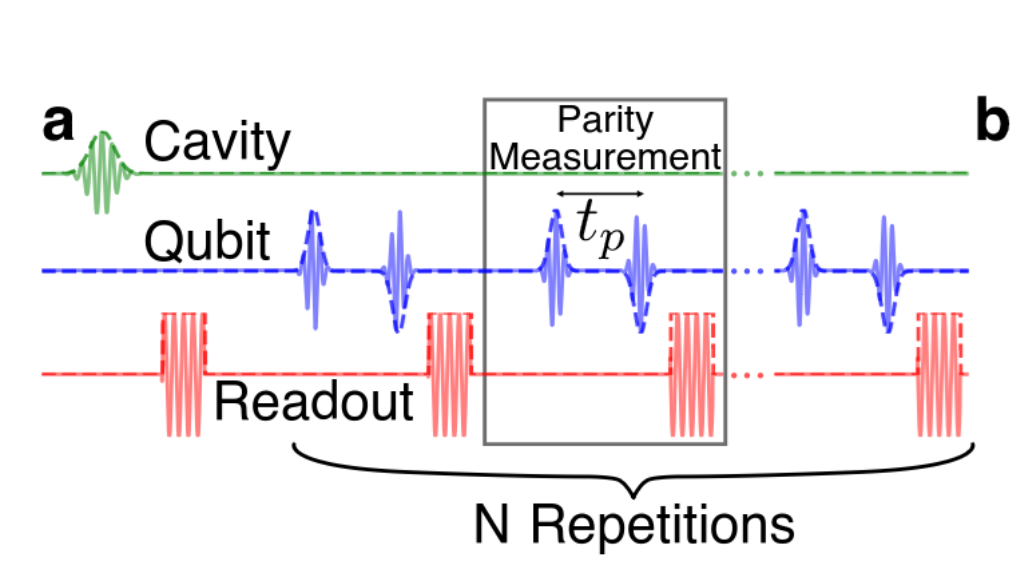
\includegraphics[width=0.6\textwidth]{Other sections/figures/dixit_sequence.png}
    \caption{Overview of the pulse sequence to be executed for the axion-detection experiment.}
    \label{fig:dixit_sequence}
\end{figure}

To increase the fidelity of the experiment, a Markov-chain analysis can be employed and it already proved to be of use.
For this example, however, we will focus on the acquisition part that can be performed using \Qibosoq, while we will leave out the data processing phase.

Using the \Qibolab and \Qibosoq API, the experimental procedure  will be coded as:

\begin{lstlisting}[language=Python, numbers=left]
from qibolab import create_platform
from qibolab.pulses import PulseSequence

# we instantiate the platform (qubit + RFSoC)
platform = create_platform("platform_name")

# we initialize an empty pulse sequence
sequence = PulseSequence()

N_repetitions = 30
for i in N_repetitions:
    # we add a first pi-half pulse
    sequence.add(platform.create_RX90_pulse())
    # we add the - pi-half pulse
    sequence.add(platform.create_RX90_pulse())
    sequence[-1].amplitude = - sequence[-1].amplitude
    # we add a measurement
    sequence.add(platform.create_MZ_pulse())

# we perform the experiment, executing the sequence
results = platform.execute_pulse_sequence(sequence)
\end{lstlisting}

See that, in 21 lines (with an abundance of comments), we coded and performed the full experiment.
Clearly, some work has been hidden here, in particular the calibration parameters of the qubit, that have to been computed via the various experiments detailed in the last sections, as well as all the data processing.

This example shows how much \Qibosoq can simplify and accelerate research.